\documentclass[a4paper, norsk, 12pt]{article}
\usepackage[utf8]{inputenc}
\usepackage[T1]{fontenc}
\usepackage{babel, textcomp, color, amsmath, amssymb, tikz, subfig, float}
\usepackage{amsfonts}
\usepackage{graphicx}
\usepackage{listings}
\usepackage{amsmath}
\usepackage[export]{adjustbox}
\usepackage[]{esint}



\begin{document}


\author{Kristian Tuv}
\title{Fys3150, Project 1}
\maketitle

\section*{Abstract}
In this project we are solving a differential equation using thre different methods. We will make a general algorithm for solving a tridiagonal matrix, we will make a specialized algorithm for a matrix with the same value on the diagonal and the same values one the subdiagonals, and we will use Armadillo's solve function\\
\\
Link to sourcecode: https://github.com/kristtuv/FYS3150/tree/master/Project1



\section*{Exercise a}
In this project we will solve the one-dimensional Poisson equation with Dirichlet boundary conditions by rewriting it as a set for linear equations.\\

We will solve the Poisson equation:\\
$$-u''(x) = f(x), \hspace{0.5cm} x\in(0,1), \hspace{0.5cm} u(0) = u(1) = 0$$\\
We approximate the second derivative of u with \\
\\
$-\dfrac{v_{i + 1} + v_{i-1} - 2v_{i}}{h^{2}} = f_{i} $,\qquad for $i = 1, ..., n$, \qquad $h = \dfrac{1}{n + 1}$, \quad $v_{0} = v_{n + 1} = 0$\\
$$ \Rightarrow - v_{i - 1} + 2v_{i} -v_{i + 1} = \underbrace{f_{i}h^{2}}_{\tilde{b}_{i}}$$\\
For $i = 1, ... , n$ and $v_{0} = v_{n + 1} = 0$ we can represent this as a set of linear equations $\mathbf{A}\mathbf{v} = \mathbf{\tilde{b}}$, with\\
\begin{equation}
    {\bf A} = \left(\begin{array}{cccccc}
                           2& -1& 0 &\dots   & \dots &0 \\
                           -1 & 2 & -1 &0 &\dots &\dots \\
                           0&-1 &2 & -1 & 0 & \dots \\
                           & \dots   & \dots &\dots   &\dots & \dots \\
                           0&\dots   &  &-1 &2& -1 \\
                           0&\dots    &  & 0  &-1 & 2 \\
                      \end{array} \right)
\end{equation}
\\
$$\mathbf{v} = \left(\begin{matrix}
v_{1}\\
v_{2}\\
\vdots\\
v_{n}
\end{matrix}\right),\qquad \mathbf{\tilde{b}} = \left(\begin{matrix}
\tilde{b}_{1}\\
\tilde{b}_{2}\\
\vdots\\
\tilde{b}_{n}
\end{matrix}\right)
$$
\\
We assue the source term of the Poisson equation is $f(x) = 100e^{-10x}$\\Which gives the solution $u(x) = 1 - (1 - e^{-10})x - e^{-10x}$\\
Taking the double derivative of $u(x)$ shows us this is a correct solution.
\\

\section*{Exercise b}
Our equation:\\
\begin{equation}
    {\bf A} = \left(\begin{array}{cccccc}
                           b_1& c_1 & 0 &\dots   & \dots &\dots \\
                           a_2 & b_2 & c_2 &\dots &\dots &\dots \\
                           & a_3 & b_3 & c_3 & \dots & \dots \\
                           & \dots   & \dots &\dots   &\dots & \dots \\
                           &   &  &a_{n-2}  &b_{n-1}& c_{n-1} \\
                           &    &  &   &a_n & b_n \\
                      \end{array} \right)\left(\begin{array}{c}
                           v_1\\
                           v_2\\
                           \dots \\
                          \dots  \\
                          \dots \\
                           v_n\\
                      \end{array} \right)
  =\left(\begin{array}{c}
                           k_1\\
                           k_2\\
                           \dots \\
                           \dots \\
                          \dots \\
                           k_n\\
                      \end{array} \right).
\end{equation}
Where I made $k_i = hf_i = \tilde{b}_{i}$ to avoid using the same letters.\\
To set up a general algorithm for solving this equation, we do a row reduction of our matrix equation. For simplicity I will use a 3x3-matrix for A and we can see the pattern.\\
\\

$\left( \begin{matrix}
 b_{1} & c_{1} & 0 & k_{1} \\
a_{2} & b_{2} & c_{2} & k_{2}\\
0 & a_{3} & b_{3} & k_{3}
\end{matrix}\right)
\sim \left(\begin{matrix}
b_{1} & c_1 & 0 & k_1\\
0 & b_2 - \dfrac{c_1a_2}{b_1} & c_2 & k_2 - \dfrac{a_2 k_1}{b_1}\\
0 & a_3 & b_3 & k_3
\end{matrix}\right)
$\\
\\


$\qquad\tilde{b}_{1} = b_1, \quad \tilde{b}_{2} = b_2 - \dfrac{c_1 a_2}{b_1}, \qquad \tilde{k}_{1} = k_1, \quad \tilde{k}_2 = fk_2 - \dfrac{a_2 k_1}{b_1}$\\
\\
\\
$\sim \left(\begin{matrix}
b_1 & c_1 & 0 & k_1\\
0 & \tilde{b}_2 & c_2 & \tilde{k}_2\\
0 & 0 & b_3 - \dfrac{c_2 a_3}{\tilde{b}_2} & k_3 - \dfrac{\tilde{k}_2 a_3}{\tilde{b}_2}
\end{matrix}\right)$\\
\\


$\tilde{b}_3 = b_3 - \dfrac{c_2 a_3}{\tilde{b}_2}, \qquad \tilde{k}_3 = f_3 - \dfrac{\tilde{k}_2 a_3}{\tilde{b}_2}$\\
\\
We now see a pattern: $\quad\tilde{b}_i = b_i - \dfrac{c_{i - 1}a_i}{\tilde{b}_{i-1}}$ and $\tilde{k}_i = k_i - \dfrac{\tilde{k}_{i - 1}a_i}{\tilde{b}_{i-1}}$\\ 
\\Which gives the matrix:\\
$$\left(\begin{matrix}
\tilde{b}_{1} & c_1 & 0 & \cdots & 0 &
 \tilde{k}_{1}\\
0 & \tilde{b}_{2} & c_2 &\cdots & 0 & \tilde{k}_2\\
0 & 0 & \ddots & \ddots  & \vdots & \vdots\\
0 &\cdots & 0 & \tilde{b}_{n-1} & c_{n-1} & \tilde{k}_{n-1}\\
0 & \cdots & \cdots & 0 & \tilde{b}_{n} & \tilde{k}_{n}\\
\end{matrix}\right)$$
\\
When we go back to our original equation, we see that\\
\\ $ v_n = \dfrac{\tilde{k}_n}{\tilde{b}_n}$ and $v_i = \dfrac{\tilde{k}_i - c_i v_{i + 1}}{\tilde{b}_i}$ for $i = n-1, ... , 1$\\

\newpage 
\subsection*{Setting up our program:}

 We now have the equations for the forward and backward substitution.\\
\textbf{Forward:} \\for i = 0:n .... \\
$\quad\tilde{b}_i = b_i - \dfrac{c_{i - 1}a_i}{\tilde{b}_{i-1}}$ \\ $\tilde{k}_i = k_i - \dfrac{\tilde{k}_{i - 1}a_i}{\tilde{b}_{i-1}}$\\
\\
\textbf{Backward:}\\
Initial:\\
$v_n = \dfrac{\tilde{k}_{n}}{\tilde{b}_{n}}$\\
\\
for i = 0:n ... \\
$v_i = \dfrac{\tilde{k}_i - c_i v_{i + 1}}{\tilde{b}_i}$\\
\\
The number of flops in this algorithm is $3n + 3n + 3n = 9n$\\


\lstset{}
\begin{lstlisting}[frame = single]
PROGRAM FLOW:

1. Declaring variables

2. Declaring vectors in matrix A
	
3. Declaring temporary vectors from the row reduction

4. Declaring initial conditions and boundary conditions

4. Forward substitution using our algorithm

5. Backward substitution using our algorithm



\end{lstlisting}

\subsection*{Results}
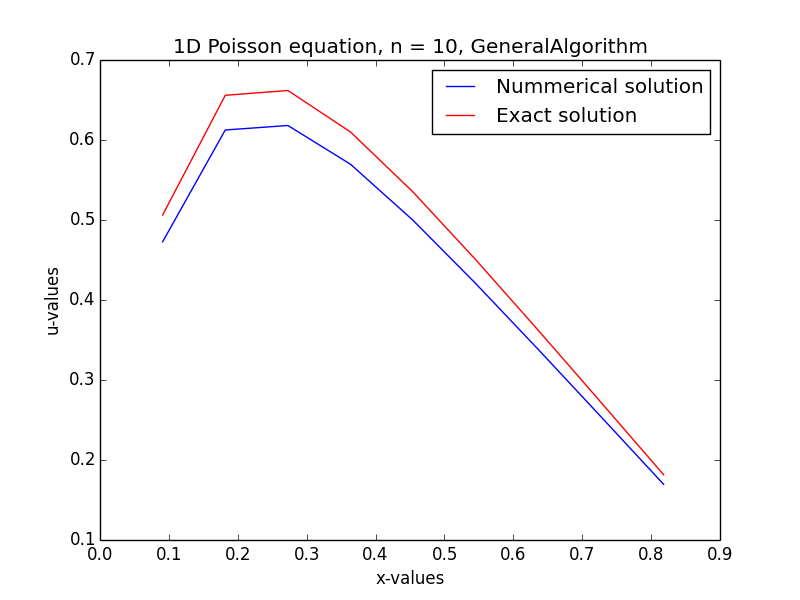
\includegraphics[scale=0.3]{/Users/Tuv/Documents/Programming/FYS3150/Project1/GeneralAlgorithm1} 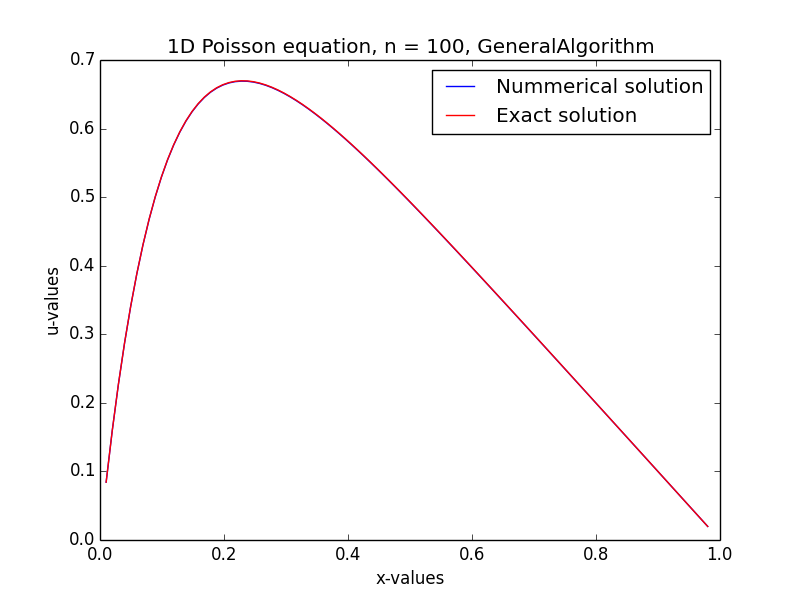
\includegraphics[scale=0.3]{/Users/Tuv/Documents/Programming/FYS3150/Project1/GeneralAlgorithm2}\\
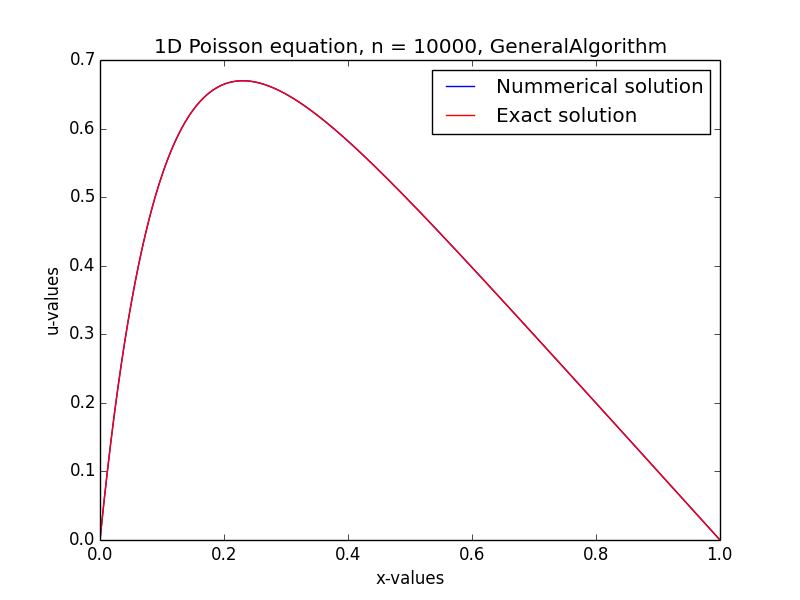
\includegraphics[scale=0.3]{/Users/Tuv/Documents/Programming/FYS3150/Project1/GeneralAlgorithm4}

Already from n = 100 we have a near perfect solution.

\section*{Exercise c}
In the specific case we can use the fact that $a_{i} = c_{i} = -1$ and $b_{i} = 2\quad \forall \quad i$\\
This means we can enter these values directly into our algorithm and decrease the number of flops.\\
 We now have the equations for the forward and backward substitution.\\
\textbf{Forward:} \\for i = 0:n .... \\
$\quad\tilde{b}_i = b_i - \frac{1}{\tilde{b}_{i-1}}$ \\ $\tilde{k}_i = k_i + \frac{\tilde{k}_{i - 1}}{\tilde{b}_{i-1}}$\\
\\
\textbf{Backward:}\\
for i = 0:n ... {\\
$v_i = \frac{\tilde{k}_i + v_{i + 1}}{\tilde{b}_i}$}\\
\\
The number of flops in this algorithm is $2n + 2n + 2n = 6n$\\
\newpage
\lstset{}
\begin{lstlisting}[frame = single]
PROGRAM FLOW:

1. Declaring variables
	
3. Declaring temporary vectors from the row reduction

4. Declaring initial conditions and boundary conditions

4. Forward substitution using our algorithm

5. Backward substitution using our algorithm

\end{lstlisting}

\section*{Exercise d}
Computing the maximum error of my general algorithm:\\
\\
\begin{tabular}{| l | r |}
\hline
n & $\epsilon_{max}$\\

\hline
$10^1$ &  -1.1797\\
$10^2$ &  -3.0880\\
$10^3$ &  -5.0800\\
$10^4$ &  -7.0793\\
$10^5$ &  -8.8883\\
$10^6$ &  -6.0755\\
$10^7$ &  -5.5520\\
\hline
\end{tabular}\\
\\
We can see that increasing n beyond  $10^5$ increases the relative error.

\section*{Exercise e}
Computing time it takes for the program to finish\\

\begin{tabular}{| r | r | r | r |}
\hline  
n & $t_{armadillo}$ (s) & $t_General$ & $t_Special$\\
\hline
$10^1$ & 0.000135 & 0.000005 &0.000002\\
$10^2$ & 0.001546 & 0.000007 &0.000024\\
$10^3$ & 0.116571 & 0.000061&0.000051\\
$10^4$ & 56.3657  & 0.00036&0.000584\\
$10^5$ & - &0.006094 &0.0044629\\
$10^6$ & - &0.050263 &0.044629\\
\hline        
\end{tabular} 
\\
\\
Because the flops in Armadillo's solver goes as $\frac{2}{3}n^{3}$, we can see that the time it takes to solve a 10000x10000 matrix is almost a minute. Running the solver for a $10^{5}\times 10^{5}$ matrix is not a good idea if you like using your computer.\\

We also see that the specialized algorithm is slightly faster, but there is basically no difference between the two as long as we do not increase n by a lot.

\section*{Conclusion}
We have shown that we get the best precision in the algorithms by using $n = 10^5$. Because the difference in flops in the general and special algorithm is relativly small, using either will take about the same amount of time. When using armadillo on the other hand, the solver takes a lot longer to finish already when $n = 10^4$, and for $n = 10^{5}$ it will be imossible to work with. The solver is not a good choice of algorithm.
\end{document}